\onecolumn
\chapter{Tabellen}

\section{Ultraviolett}
\begin{table}[h!]
    \centering
    \begin{tabular}{c | ccc}
    \hline
    $U [V]$ & $U_I \, [\mathrm{V}]$ & $U_{\text{diff}} \, [\mathrm{V}]$ & $\sqrt{U_{\text{diff}}} \, [\mathrm{\sqrt{V}}]$ \\
    \hline
    $0,30$ & $2,392 \pm 0,015$ & $1,547 \pm 0,019$ & $1,244 \pm 0,012$ \\
    $0,20$ & $2,215 \pm 0,015$ & $1,488 \pm 0,018$ & $1,220 \pm 0,011$ \\
    $0,10$ & $2,056 \pm 0,015$ & $1,434 \pm 0,018$ & $1,198 \pm 0,011$ \\
    $0,00$ & $2,086 \pm 0,015$ & $1,444 \pm 0,018$ & $1,202 \pm 0,011$ \\
    $-0,10$ & $1,902 \pm 0,015$ & $1,379 \pm 0,018$ & $1,174 \pm 0,010$ \\
    $-0,20$ & $1,742 \pm 0,015$ & $1,320 \pm 0,018$ & $1,149 \pm 0,010$ \\
    $-0,30$ & $1,585 \pm 0,015$ & $1,259 \pm 0,017$ & $1,122 \pm 0,010$ \\
    $-0,40$ & $1,436 \pm 0,015$ & $1,198 \pm 0,017$ & $1,095 \pm 0,009$ \\
    $-0,50$ & $1,292 \pm 0,015$ & $1,137 \pm 0,017$ & $1,066 \pm 0,009$ \\
    $-0,60$ & $1,142 \pm 0,014$ & $1,069 \pm 0,017$ & $1,034 \pm 0,009$ \\
    $-0,70$ & $1,007 \pm 0,014$ & $1,003 \pm 0,017$ & $1,002 \pm 0,008$ \\
    $-0,80$ & $0,875 \pm 0,014$ & $0,935 \pm 0,017$ & $0,967 \pm 0,008$ \\
    $-0,90$ & $0,740 \pm 0,014$ & $0,860 \pm 0,016$ & $0,927 \pm 0,008$ \\
    $-1,00$ & $0,624 \pm 0,014$ & $0,790 \pm 0,016$ & $0,889 \pm 0,007$ \\
    $-1,10$ & $0,507 \pm 0,014$ & $0,712 \pm 0,016$ & $0,844 \pm 0,007$ \\
    $-1,20$ & $0,392 \pm 0,014$ & $0,626 \pm 0,016$ & $0,791 \pm 0,006$ \\
    $-1,30$ & $0,303 \pm 0,014$ & $0,550 \pm 0,016$ & $0,741 \pm 0,006$ \\
    $-1,40$ & $0,223 \pm 0,014$ & $0,472 \pm 0,016$ & $0,687 \pm 0,005$ \\
    $-1,50$ & $0,158 \pm 0,014$ & $0,397 \pm 0,016$ & $0,630 \pm 0,005$ \\
    $-1,60$ & $0,110 \pm 0,014$ & $0,332 \pm 0,016$ & $0,576 \pm 0,005$ \\
    $-1,70$ & $0,066 \pm 0,014$ & $0,257 \pm 0,016$ & $0,507 \pm 0,004$ \\
    $-1,80$ & $0,035 \pm 0,014$ & $0,187 \pm 0,016$ & $0,432 \pm 0,003$ \\
    $-4,00$ & $-(0,012 \pm 0,010)$ & & \\
    \hline
    \end{tabular}
    \caption{Messwerte für ultraviolettes Licht: $U [V]$, Photostrom $U_I [V]$, Differenzspannung $U_{diff} [V]$ und deren Quadratwurzel.}
    \label{tab:uv_values}
\end{table}


\newpage

\section{Violett}
\begin{table}[h!]
    \centering
    \begin{tabular}{cccc}
    \hline
    $U [V]$ & $U_I \, [\mathrm{V}]$ & $U_{\text{diff}} \, [\mathrm{V}]$ & $\sqrt{U_{\text{diff}}} \, [\mathrm{\sqrt{V}}]$ \\
    \hline
    $0,30$ & $2,262 \pm 0,015$ & $1,504 \pm 0,018$ & $1,227 \pm 0,011$ \\
    $0,20$ & $2,089 \pm 0,015$ & $1,445 \pm 0,018$ & $1,202 \pm 0,011$ \\
    $0,10$ & $1,914 \pm 0,015$ & $1,383 \pm 0,018$ & $1,176 \pm 0,011$ \\
    $0,00$ & $1,755 \pm 0,015$ & $1,325 \pm 0,018$ & $1,151 \pm 0,010$ \\
    $-0,10$ & $1,570 \pm 0,015$ & $1,253 \pm 0,017$ & $1,120 \pm 0,010$ \\
    $-0,20$ & $1,413 \pm 0,015$ & $1,189 \pm 0,017$ & $1,091 \pm 0,009$ \\
    $-0,30$ & $1,260 \pm 0,014$ & $1,122 \pm 0,017$ & $1,059 \pm 0,009$ \\
    $-0,40$ & $1,125 \pm 0,014$ & $1,061 \pm 0,017$ & $1,030 \pm 0,009$ \\
    $-0,50$ & $0,980 \pm 0,014$ & $0,990 \pm 0,017$ & $0,995 \pm 0,008$ \\
    $-0,60$ & $0,839 \pm 0,014$ & $0,916 \pm 0,017$ & $0,957 \pm 0,008$ \\
    $-0,70$ & $0,694 \pm 0,014$ & $0,833 \pm 0,016$ & $0,912 \pm 0,007$ \\
    $-0,80$ & $0,568 \pm 0,014$ & $0,754 \pm 0,016$ & $0,868 \pm 0,007$ \\
    $-0,90$ & $0,440 \pm 0,014$ & $0,663 \pm 0,016$ & $0,814 \pm 0,007$ \\
    $-1,00$ & $0,325 \pm 0,014$ & $0,570 \pm 0,016$ & $0,755 \pm 0,006$ \\
    $-1,10$ & $0,232 \pm 0,014$ & $0,482 \pm 0,016$ & $0,694 \pm 0,006$ \\
    $-1,20$ & $0,157 \pm 0,014$ & $0,396 \pm 0,016$ & $0,629 \pm 0,005$ \\
    $-1,30$ & $0,100 \pm 0,014$ & $0,316 \pm 0,016$ & $0,562 \pm 0,004$ \\
    $-1,40$ & $0,053 \pm 0,014$ & $0,230 \pm 0,016$ & $0,480 \pm 0,004$ \\
    $-4,00$ & $-(0,010 \pm 0,010)$ & & \\
    \hline
    \end{tabular}
    \caption{Messwerte für violettes Licht: $U [V]$, Photostrom $U_I [V]$, Differenzspannung $U_{diff} [V]$ und deren Quadratwurzel.}
    \label{tab:violett_values}
\end{table}



\newpage

\section{Blau}
\begin{table}[h!]
    \centering
    \begin{tabular}{cccc}
    \hline
    $U [V]$ & $U_I \, [\mathrm{V}]$ & $U_{\text{diff}} \, [\mathrm{V}]$ & $\sqrt{U_{\text{diff}}} \, [\mathrm{\sqrt{V}}]$ \\
    \hline
    $0,30$ & $3,648 \pm 0,017$ & $1,9100 \pm 0,021$ & $1,382 \pm 0,014$ \\
    $0,20$ & $3,354 \pm 0,016$ & $1,83139 \pm 0,020$ & $1,354 \pm 0,014$ \\
    $0,10$ & $3,053 \pm 0,016$ & $1,7473 \pm 0,020$ & $1,322 \pm 0,013$ \\
    $0,00$ & $2,787 \pm 0,016$ & $1,66943 \pm 0,019$ & $1,292 \pm 0,012$ \\
    $-0,10$ & $2,491 \pm 0,015$ & $1,578 \pm 0,019$ & $1,256 \pm 0,012$ \\
    $-0,20$ & $2,230 \pm 0,015$ & $1,493 \pm 0,018$ & $1,222 \pm 0,011$ \\
    $-0,30$ & $1,944 \pm 0,015$ & $1,394 \pm 0,018$ & $1,180 \pm 0,011$ \\
    $-0,40$ & $1,674 \pm 0,015$ & $1,294 \pm 0,018$ & $1,138 \pm 0,010$ \\
    $-0,50$ & $1,396 \pm 0,015$ & $1,182 \pm 0,017$ & $1,087 \pm 0,009$ \\
    $-0,60$ & $1,136 \pm 0,014$ & $1,066 \pm 0,017$ & $1,033 \pm 0,009$ \\
    $-0,70$ & $0,915 \pm 0,014$ & $0,957 \pm 0,017$ & $0,978 \pm 0,008$ \\
    $-0,80$ & $0,701 \pm 0,014$ & $0,837 \pm 0,016$ & $0,915 \pm 0,008$ \\
    $-0,90$ & $0,503 \pm 0,014$ & $0,709 \pm 0,016$ & $0,842 \pm 0,007$ \\
    $-1,00$ & $0,329 \pm 0,014$ & $0,574 \pm 0,016$ & $0,758 \pm 0,006$ \\
    $-1,10$ & $0,198 \pm 0,014$ & $0,445 \pm 0,016$ & $0,667 \pm 0,005$ \\
    $-1,20$ & $0,118 \pm 0,014$ & $0,344 \pm 0,016$ & $0,586 \pm 0,005$ \\
    $-1,30$ & $0,048 \pm 0,014$ & $0,219 \pm 0,016$ & $0,468 \pm 0,004$ \\
    $-4,00$ & $-(0,009 \pm 0,010)$ & & \\
    \hline
    \end{tabular}
    \caption{Messwerte für blaues Licht: $U [V]$, Photostrom $U_I [V]$, Differenzspannung $U_{diff} [V]$ und deren Quadratwurzel.}
    \label{tab:blau_values}
\end{table}


\newpage

\section{Grün}
\begin{table}[h!]
    \centering
    \begin{tabular}{cccc}
    \hline
    $U [V]$ & $U_I \, [\mathrm{V}]$ & $U_{\text{diff}} \, [\mathrm{V}]$ & $\sqrt{U_{\text{diff}}} \, [\mathrm{\sqrt{V}}]$ \\
    \hline
    $0,30$ & $4,649 \pm 0,023$ & $2,156 \pm 0,024$ & $1,468 \pm 0,018$ \\
    $0,20$ & $4,119 \pm 0,022$ & $2,030 \pm 0,022$ & $1,425 \pm 0,016$ \\
    $0,10$ & $3,607 \pm 0,017$ & $1,8992 \pm 0,021$ & $1,378 \pm 0,014$ \\
    $0,00$ & $3,096 \pm 0,016$ & $1,7595 \pm 0,020$ & $1,326 \pm 0,013$ \\
    $-0,10$ & $2,547 \pm 0,016$ & $1,596 \pm 0,019$ & $1,263 \pm 0,012$ \\
    $-0,20$ & $1,974 \pm 0,015$ & $1,405 \pm 0,018$ & $1,186 \pm 0,011$ \\
    $-0,30$ & $1,568 \pm 0,015$ & $1,252 \pm 0,017$ & $1,118 \pm 0,010$ \\
    $-0,40$ & $1,359 \pm 0,015$ & $1,166 \pm 0,017$ & $1,080 \pm 0,009$ \\
    $-0,50$ & $0,758 \pm 0,014$ & $0,871 \pm 0,016$ & $0,933 \pm 0,008$ \\
    $-0,60$ & $0,440 \pm 0,014$ & $0,663 \pm 0,016$ & $0,814 \pm 0,007$ \\
    $-0,70$ & $0,200 \pm 0,014$ & $0,447 \pm 0,016$ & $0,669 \pm 0,005$ \\
    $-0,80$ & $0,066 \pm 0,014$ & $0,257 \pm 0,016$ & $0,507 \pm 0,004$ \\
    $-0,85$ & $0,032 \pm 0,014$ & $0,1789 \pm 0,016$ & $0,423 \pm 0,003$ \\
    $-4,00$ & $-(0,009 \pm 0,010)$ & & \\
    \hline
    \end{tabular}
    \caption{Messwerte für grünes Licht: $U [V]$, Photostrom $U_I [V]$, Differenzspannung $U_{diff} [V]$ und deren Quadratwurzel.}
    \label{tab:gruen_values}
\end{table}


\newpage

\section{Gelb}
\begin{table}[h!]
    \centering
    \begin{tabular}{cccc}
    \hline
    $U [V]$ & $U_I \, [\mathrm{V}]$ & $U_{\text{diff}} \, [\mathrm{V}]$ & $\sqrt{U_{\text{diff}}} \, [\mathrm{\sqrt{V}}]$ \\
    \hline
    $0,30$ & $3,549 \pm 0,017$ & $1,8839 \pm 0,020$ & $1,373 \pm 0,014$ \\
    $0,20$ & $2,993 \pm 0,016$ & $1,7300 \pm 0,019$ & $1,315 \pm 0,013$ \\
    $0,10$ & $2,512 \pm 0,015$ & $1,585 \pm 0,019$ & $1,259 \pm 0,012$ \\
    $0,00$ & $2,017 \pm 0,015$ & $1,420 \pm 0,018$ & $1,192 \pm 0,011$ \\
    $-0,10$ & $1,588 \pm 0,015$ & $1,260 \pm 0,017$ & $1,122 \pm 0,010$ \\
    $-0,20$ & $1,179 \pm 0,014$ & $1,086 \pm 0,017$ & $1,042 \pm 0,009$ \\
    $-0,30$ & $0,808 \pm 0,014$ & $0,899 \pm 0,017$ & $0,948 \pm 0,008$ \\
    $-0,40$ & $0,491 \pm 0,014$ & $0,701 \pm 0,016$ & $0,837 \pm 0,007$ \\
    $-0,50$ & $0,255 \pm 0,014$ & $0,505 \pm 0,016$ & $0,711 \pm 0,006$ \\
    $-0,60$ & $0,114 \pm 0,014$ & $0,338 \pm 0,016$ & $0,581 \pm 0,005$ \\
    $-0,70$ & $0,037 \pm 0,014$ & $0,192 \pm 0,016$ & $0,438 \pm 0,003$ \\
    $-4,00$ & $-(0,007 \pm 0,010)$ & & \\
    \hline
    \end{tabular}
    \caption{Messwerte für gelbes Licht: $U [V]$, Photostrom $U_I [V]$, Differenzspannung $U_{diff} [V]$ und deren Quadratwurzel.}
    \label{tab:gelb_values}
\end{table}

\newpage
% \chapter{Graphen}

\begin{figure}[t!]
    % \raggedright
    % \hspace*{-2.2cm}
    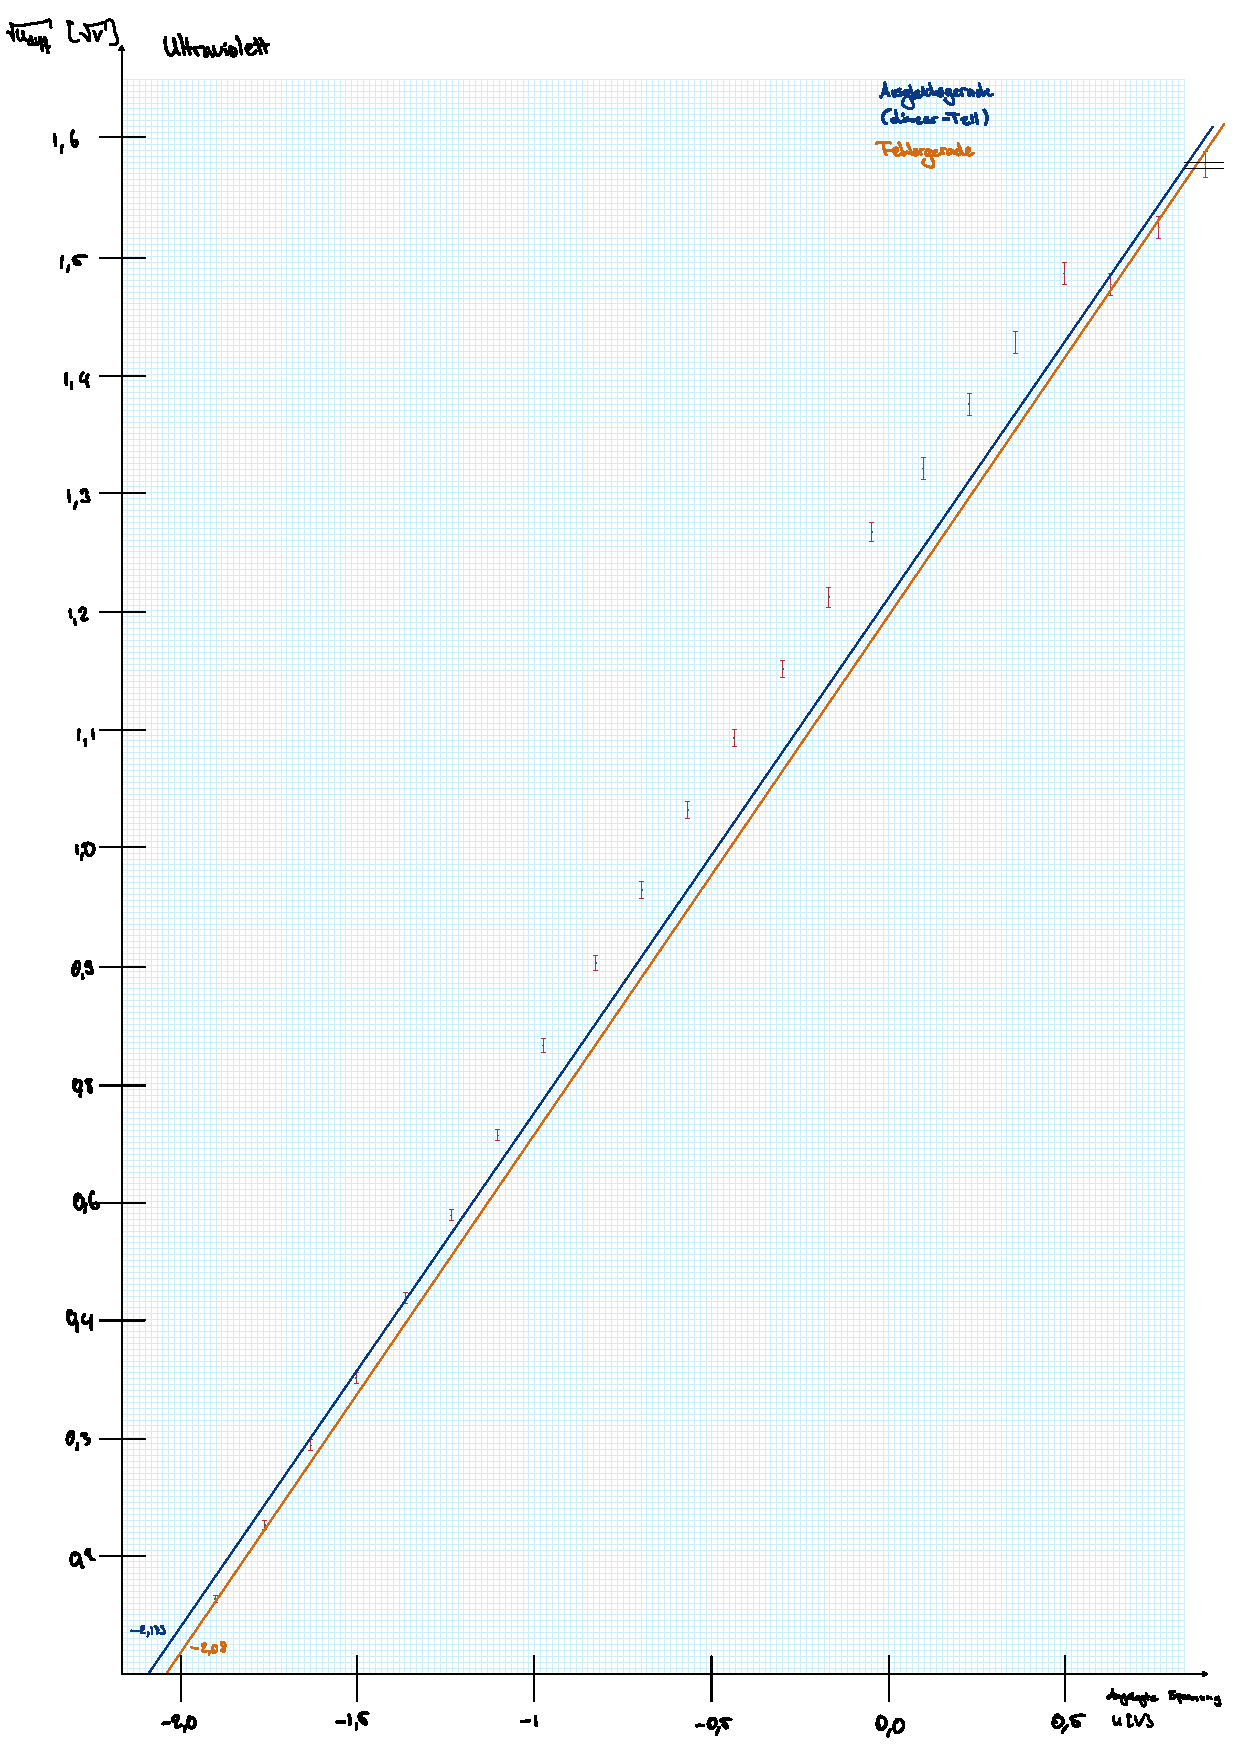
\includegraphics[width=1\textwidth, page=1]{img/35/v35-Farbplots.pdf}
    \caption{Bestimmung der Sperrspannung für die Spektrallinie im UV-Bereich}
    \label{fig:uv}
\end{figure}

\newpage

\begin{figure}[t!]
    % \raggedright
    % \hspace*{-2.2cm}
    \includegraphics[width=1\textwidth, page=2]{img/35/v35-Farbplots.pdf}
    \caption{Bestimmung der Sperrspannung für die Spektrallinie für violettes Licht}
    \label{fig:v}
\end{figure}

\newpage

\begin{figure}[t!]
    % \raggedright
    % \hspace*{-2.2cm}
    \includegraphics[width=1\textwidth, page=3]{img/35/v35-Farbplots.pdf}
    \caption{Bestimmung der Sperrspannung für die Spektrallinie für blaues Licht}
    \label{fig:b}
\end{figure}

\newpage

\begin{figure}[t!]
    % \raggedright
    % \hspace*{-2.2cm}
    \includegraphics[width=1\textwidth, page=4]{img/35/v35-Farbplots.pdf}
    \caption{Bestimmung der Sperrspannung für die Spektrallinie für grünes Licht}
    \label{fig:gr}
\end{figure}

\newpage

\begin{figure}[t!]
    % \raggedright
    % \hspace*{-2.2cm}
    \includegraphics[width=1\textwidth, page=5]{img/35/v35-Farbplots.pdf}
    \caption{Bestimmung der Sperrspannung für die Spektrallinie für gelbes Licht}
    \label{fig:gl}
\end{figure}

\newpage

\begin{figure}[t!]
    % \raggedright
    % \hspace*{-2.2cm}
    \includegraphics[width=1\textwidth, page=6]{img/35/v35-Farbplots.pdf}
    \caption{estimmung des Plank'schen Wirkungsquantums}
    \label{fig:final}
\end{figure}

\twocolumn